\chapter{Results and Discussion}
\label{ch:results}

\section{As-Recieved Membranes}
\subsection{Fouling profiles of the as-received membranes}
\label{sec:res-fouling}
The conditions of the three EoL elements before treatment was established by the Membrane Work autopsies \citep{MembraneWorks2026Mine,MembraneWorks2025Desal}, and summarised in Table~\ref{tab:eol-summary}. All three were lightly fouled, but they differed in the state of their PA layer.

\paragraph{Desal-site first-pass element (4238A).}
\label{sec:red-fouling-4238A}
4238A was in good condition and still met the specifications of the element. Deposits were mainly light iron and aluminosilicate (clay) particles, and FTIR spectrum matched the new element. Dye test showed minor pinholing similar to that of new elements \citep{MembraneWorks2025Desal}. It displayed a lower contact angle, attributed to adsorbed organic or biological material. 

\paragraph{Desal-site second-pass element (4238C).}
\label{sec:res-fouling-4238C}
The main problem with 4238C was damaged to the PA layer, not fouling. Deposits were limited to patches of iron oxide, some biological material and NaCl crystals. FTIR showed no chemical difference from new element \citep{MembraneWorks2025Desal}. However, SEM showed holes in teh PA layer across the surface, which were also seen at higher magnification in this thesis (Figure~\ref{fig:app_sem_4238C_eol}). The dye test confirms this, with dense spots and streaks of dye on the permeate side (Figure~\ref{fig:dye_test_full}). The surface also became less negatively charged and more hydrophillic over service. Similar charge loss had also been reported for membranes cleaned repeatedly with caustic \citep{MembraneWorks2025Desal}, and the pH~10 feed may have had a similar effect.


\begin{figure}[htbp]
    \centering
    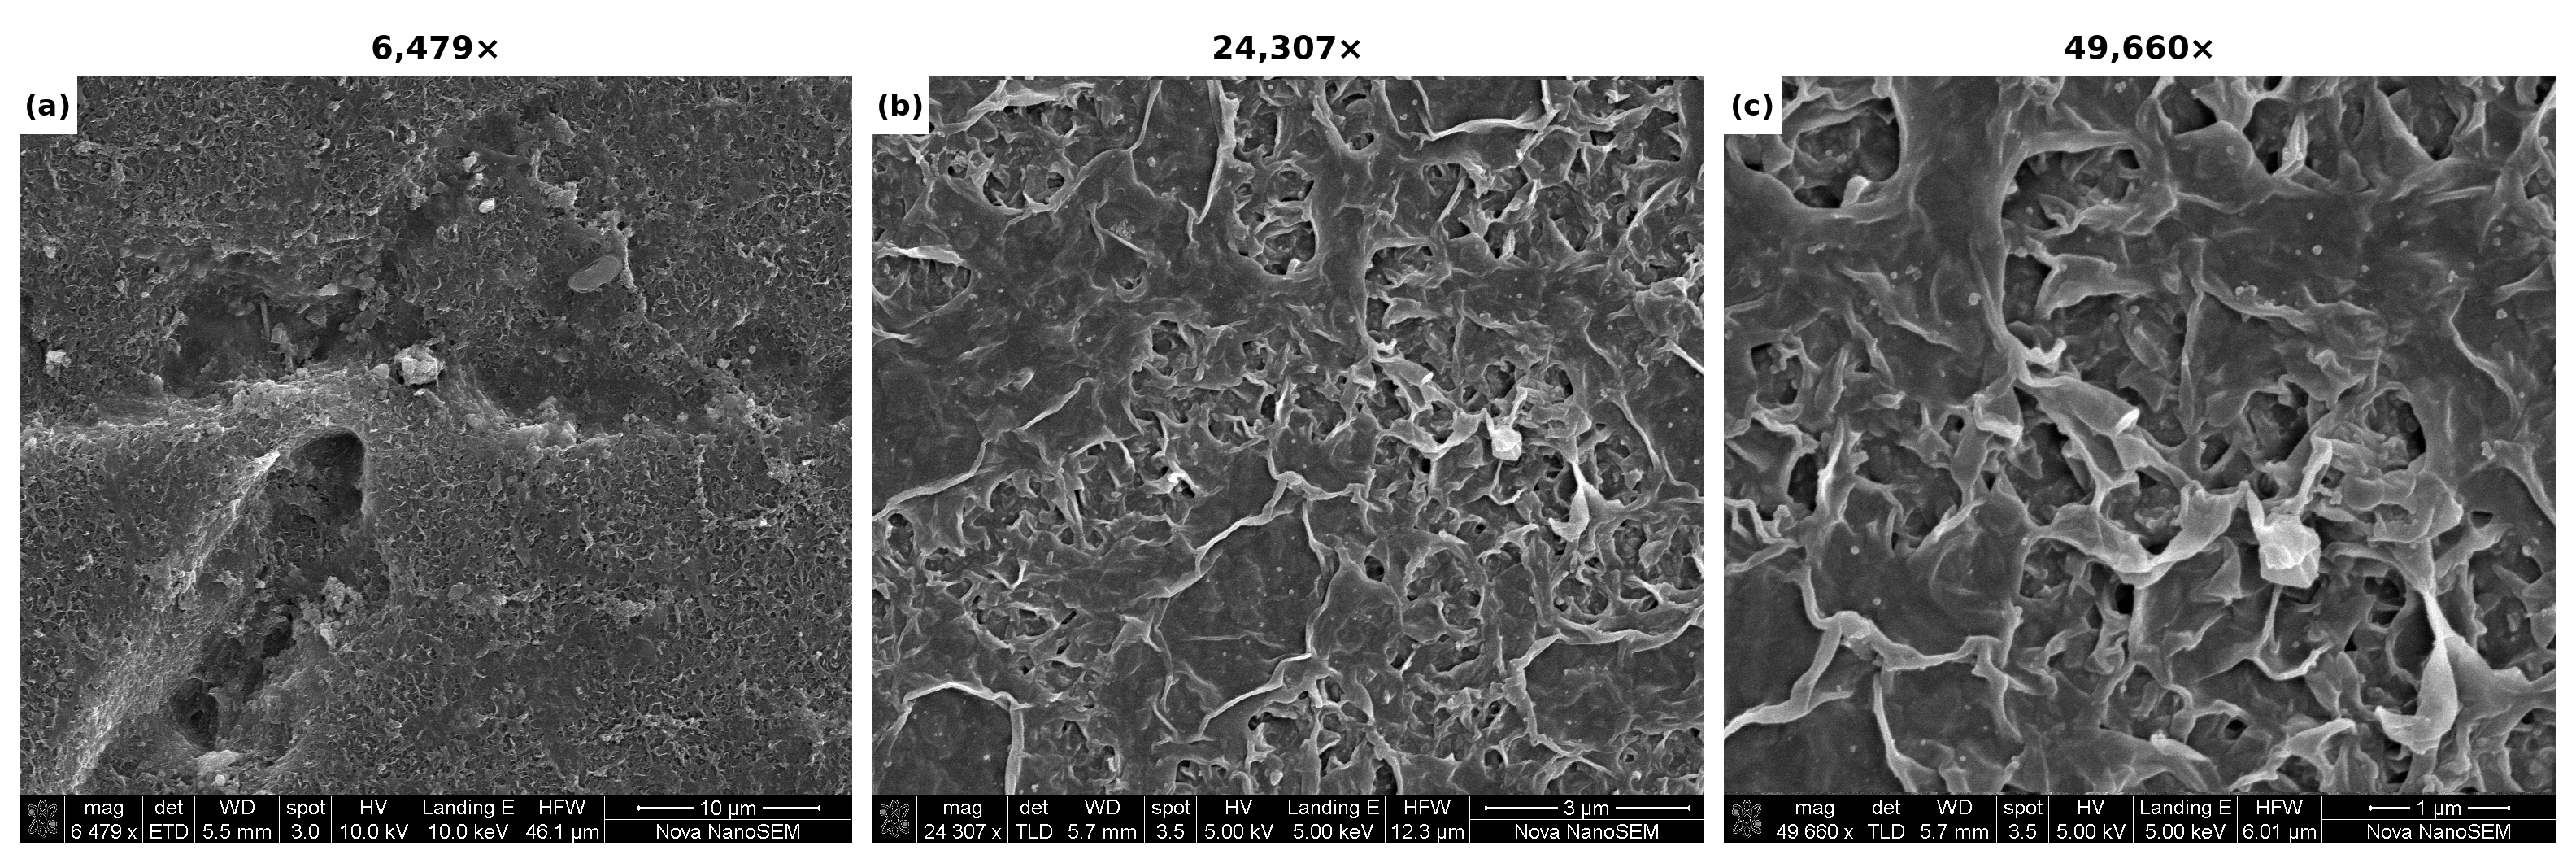
\includegraphics[width=\textwidth]{figures/Analysis/SEM/Fig_4238C_EoL_SEM.png}
    \caption{SEM micrographs of the end-of-life (as received) 4238C membrane
    surface at (a) 6,479$\times$, (b) 24,307$\times$ and (c) 49,660$\times$,
    showing damage to the polyamide layer.}
    \label{fig:sem_4238C_eol}
\end{figure}


\begin{figure}[htbp]
  \centering
  \setlength{\tabcolsep}{3pt}
  \renewcommand{\arraystretch}{1.1}
  \begin{tabular}{>{\centering\arraybackslash}m{0.16\linewidth}
                  >{\centering\arraybackslash}m{0.28\linewidth}
                  >{\centering\arraybackslash}m{0.28\linewidth}}
    \toprule
    \textbf{Membrane} & \textbf{Feed side} & \textbf{Permeate side} \\
    \midrule
    Used 2\textsuperscript{nd} pass \newline (4238C) &
      \includegraphics[width=\linewidth]{figures/dye_test/full_4238C_feed} &
      \includegraphics[width=\linewidth]{figures/dye_test/full_4238C_permeate} \\[2pt]
    New 2\textsuperscript{nd} pass \newline (4238D) &
      \includegraphics[width=\linewidth]{figures/dye_test/full_4238D_feed} &
      \includegraphics[width=\linewidth]{figures/dye_test/full_4238D_permeate} \\
    \bottomrule
  \end{tabular}
  \caption[Dye integrity test of desalination site membrane coupons]{Dye integrity test of desalination site membrane coupons, showing the feed side (left) and permeate side (right). Dye on the permeate side indicates passage through defects in the polyamide layer. Adapted from \citep{MembraneWorks2025Desal}.}
  \label{fig:dye_test_full}
\end{figure}



\paragraph{Mine-site element (4297B).}
4297B had a light brown fouling layer across the surface. SEM-EDS showed scattered iron and silica particles. Astra Blue staining and bacterial counts indicated moderate biofouling \citep{MembraneWorks2026Mine}. Only a small amount of foulant could be extracted by acid and caustic, mainly calcium, magnesium and sulphate. These foulant types are consistent with the high calcium and sulphate feed. Almost no iron was extracted, even though both were visible in SEM-EDS, so these deposits resisted acid and caustic. Foulants had also penetrated into the support layers, and scale had left some indentation on the surface. XPS also detected low-level chlorine damage, but the PA layer was otherwise mostly intact. There was a reported drop to about \qty{85}{\percent} rejection measured across the whole RO train \citep{MembraneWorks2026Mine},

\begin{table}[htbp]
  \centering
  \caption{Summary of the as-received condition of the three EoL elements \citep{MembraneWorks2025Desal,MembraneWorks2026Mine}.}
  \label{tab:eol-summary}
  \small
  \begin{tabularx}{\textwidth}{@{}>{\raggedright\arraybackslash}p{0.17\textwidth}*{3}{>{\raggedright\arraybackslash}X}@{}}
    \toprule
    & \textbf{4238A} & \textbf{4238C} & \textbf{4297B} \\
    \midrule
    Service & Desal, 1st pass, neutral pH, 4.5~years
            & Desal, 2nd pass, pH~10 feed, 4.5~years
            & Mine site, high Ca and sulphate feed \\
    \addlinespace
    Main deposits (SEM-EDS) & Fe with aluminosilicate clay (up to 13 at.\% Fe, 12 at.\% Si, 11 at.\% Al)
            & Patchy Fe oxide (up to 30.9 at.\% Fe), biological material (up to 14.3 at.\% N), NaCl crystals
            & Fe oxide (37.3 at.\% Fe), silica (29.6 at.\% Si), low N (5.4 at.\%) \\
    \addlinespace
    Extractable foulant (\unit{mg.m^{-2}}) & Not tested & Not tested
            & 237.5 total: Ca 91, Mg 30, S 26, Si 10, Fe $\leq 1$ \\
    \addlinespace
    Biofouling & Minor & Moderate
            & Moderate (5800--7800~CFU/mL); EPS under brine spacer \\
    \addlinespace
    Element flux; rejection (spec.) & \qty{26.6}{LMH} (22.1); \qty{99.65}{\percent} (99.68)
            & \qty{71.9}{LMH} (37.3); \qty{97.3}{\percent} (99.46)
            & Not tested; train rejection fell to $\sim$\qty{85}{\percent} \\
    \addlinespace
    Dye test & Minor pinholing at spacer contact, as for new elements
            & Heavy dye passage; permeate \qty{113}{\micro\siemens\per\centi\metre} (others 20--30)
            & Not tested \\
    \addlinespace
    PA condition & Intact; FTIR matches new element
            & Holes across surface (SEM); FTIR matches new element
            & Mostly intact; 0.2 at.\% organic Cl (XPS); scale indentations; foulant in support layers \\
    \addlinespace
    Contact angle (\unit{\degree}) & 25.1 (new: 44.2) & 34.5 (new: 58.5) & Not tested \\
    \addlinespace
    Zeta potential at pH~7 (\unit{mV}) & $-30$ (new: $-8$) & $-16$ (new: $-42$) & Not tested \\
    \addlinespace
    Main issue & None & PA damage & Fouling and scaling \\
    \bottomrule
  \end{tabularx}
  \par\smallskip
  \footnotesize Element tests at \qty{1500}{\milli\gram\per\litre} NaCl and \qty{10}{bar}. Extractable foulant from acid and caustic extraction.
\end{table}

%-------------------––––Next Section-----------------%
\subsection{Performance of the as-received membranes}
\label{sec:res-baseline}
As-received coupons were tested on the crossflow rig to give a baseline for each membrane (Table~\ref{tab:baseline}). Later results are compared against these values.

  \begin{table}[htbp]
  \centering
  \caption{Performance of the as-received membranes (no clean, no IP). Mean $\pm$ SD across coupons.}
  \label{tab:baseline}
    \begin{tabular}{llcccc}
    \toprule
    Campaign & Membrane & Flux (\unit{LMH}) & PWP (\unit{LMH.bar^{-1}}) & NaCl rejection (\%) & $n$ \\
    \midrule
    1 & 4238A (desal) & $1.23 \pm 0.27$ & $0.082 \pm 0.018$ & $78.1 \pm 2.8$ & 2 \\
    2 & 4238C (desal) & $3.21 \pm 0.32$ & $0.208 \pm 0.011$ & $76.6 \pm 3.1$ & 4 \\
    2 & 4297B (mine)  & $5.22 \pm 1.00$ & $0.330 \pm 0.062$ & $81.9 \pm 8.6$ & 4 \\
    \bottomrule
  \end{tabular}
  \par\smallskip
  \footnotesize $n$ = number of coupons. Flux and PWP at \qtyrange{14.3}{16.3}{bar}; rejection with $\sim$\qty{2000}{\milli\gram\per\litre} NaCl (\qtyrange{3800}{4000}{\micro\siemens\per\centi\metre}).
  \end{table}

Coupon results were consistently far below the element results reported by \citet{MembraneWorks2025Desal}. As an element, 4238A met specification with \qty{99.65}{\percent} NaCl rejection. As a coupon it rejected only \qty{78.1}{\percent}. 4238C showed a similar gap, with \qty{76.6}{\percent} as a coupon against \qty{97.3}{\percent} as an element. Coupon permeability was also about 32--35 times lower than the element values. The elements gave roughly \qty{2.6}{} and \qty{7.2}{LMH.bar^{-1}} at \qty{10}{bar}, while the 4238A coupon gave only \qty{0.082}{LMH.bar^{-1}}. No element test was done for 4297B. Its reported drop to around \qty{85}{\percent} rejection was measured across the whole RO train \citep{MembraneWorks2026Mine}.

PA damage could explain part of the result for 4238C, where the element flux was about double the expected \qty{37.3}{LMH}, and its dye-cell rejection was \qty{61}{\percent}, against \qtyrange{91}{92}{\percent} for the other coupons. Damage cannot explain 4238A, which was intact as an element yet performed almost the same as 4238C on the rig. The offset therefore comes mainly from the test method. First, at constant salt permeability, observed rejection falls with water flux, and coupon fluxes (\qtyrange{1.0}{6.5}{LMH}) were an order of magnitude below element fluxes. Second, salt may leak through local defects or past the O-ring seal. On a \qty{0.0139}{\square\metre} coupon this has a much larger effect than across a full element.

This offset applies to every test on the rig, so while comparisons between conditions remain valid, these values should not be compared with element or datasheet values.

%-------------------––––Next Section-----------------%
\section{Cleaning outcomes}
\label{sec:res-cleaning}
This section reports the effect of cleaning on each membrane. The effect of cleaning on regeneration is covered in Section~\ref{sec:res-cleaning-effect}. Based on the autopsies, cleaning is not expected to repair the PA damage on 4238C or to remove the iron oxide and silica foulants on 4297B. On 4297B, the alkaline step is expected to remove the organic and biological material, with EDTA breaking the calcium bridges \citep{Ang2006}, and the acid step expected to remove calcium, magnesium and sulphates. Iron oxide was expected to remain, since even specialist iron cleaner at up to \qty{4}{\percent} did not fully remove it in Membrane Work's cleaning study \citep{MembraneWorks2026Mine}.
% --------------------------------------------------------------------


\subsection{Visual observations}
\paragraph{Desal-site membrane 4238C and 4238A. } 
Cleaning caused no visible change to both 4238C and 4238A. Before cleaning, the polyamide (feed side) was a shiny, light yellow colour for 4238C, and a darker orange shade for 4238A. The polyester (permeate side) for both was a dull, matte white. After acid and base cleans, the coupon looked exactly the same. The acid and base solutions also showed no colour change after use. This could suggests that little foulant was dissolved into the solutions.

\paragraph{Mine-site membrane 4297B.}
The colour of 4297B did not change noticeably after cleaning. The acid and base solutions also showed no colour change. 

The main observation for 4297B was delamination along the edges of the coupons (Figure~\ref{fig:4297B-delam}). In these areas the PA layer had begun to peel away from the polysulfone support and could be lifted off with very little force. The damage was first seen immediately after the base clean and appeared again in repeated experiments.The autopsy found no delamination damage on the EoL 4297B elements, so the damage was not there before cleaning. 4238C showed no delamination under the same cleaning conditions, so cleaning itself doesn't cause this. 

The base clean reached pH values up to 11.5. This is slightly above the manufacturer's limit for continuous operation (pH~2--11) but within the short-term (\qty{30}{\minute}) cleaning range (pH~1--13) \citep{MembraneWorks2026Mine}. Since 4238C was not affected at the same pH, the more likely explanation is that the bond between the PA and the support in 4297B had already weakened during service. The autopsy found that foulants had penetrated into the support layers of 4297B, and indentations left on the surface by past scale may also have weakened the layer adhesion.

The damage was concentrated along the coupon edges and were therefore trimmed off and discarded before testing.

\begin{figure}[htbp]
  \centering
  \begin{minipage}[b]{0.36\linewidth}
    \centering
    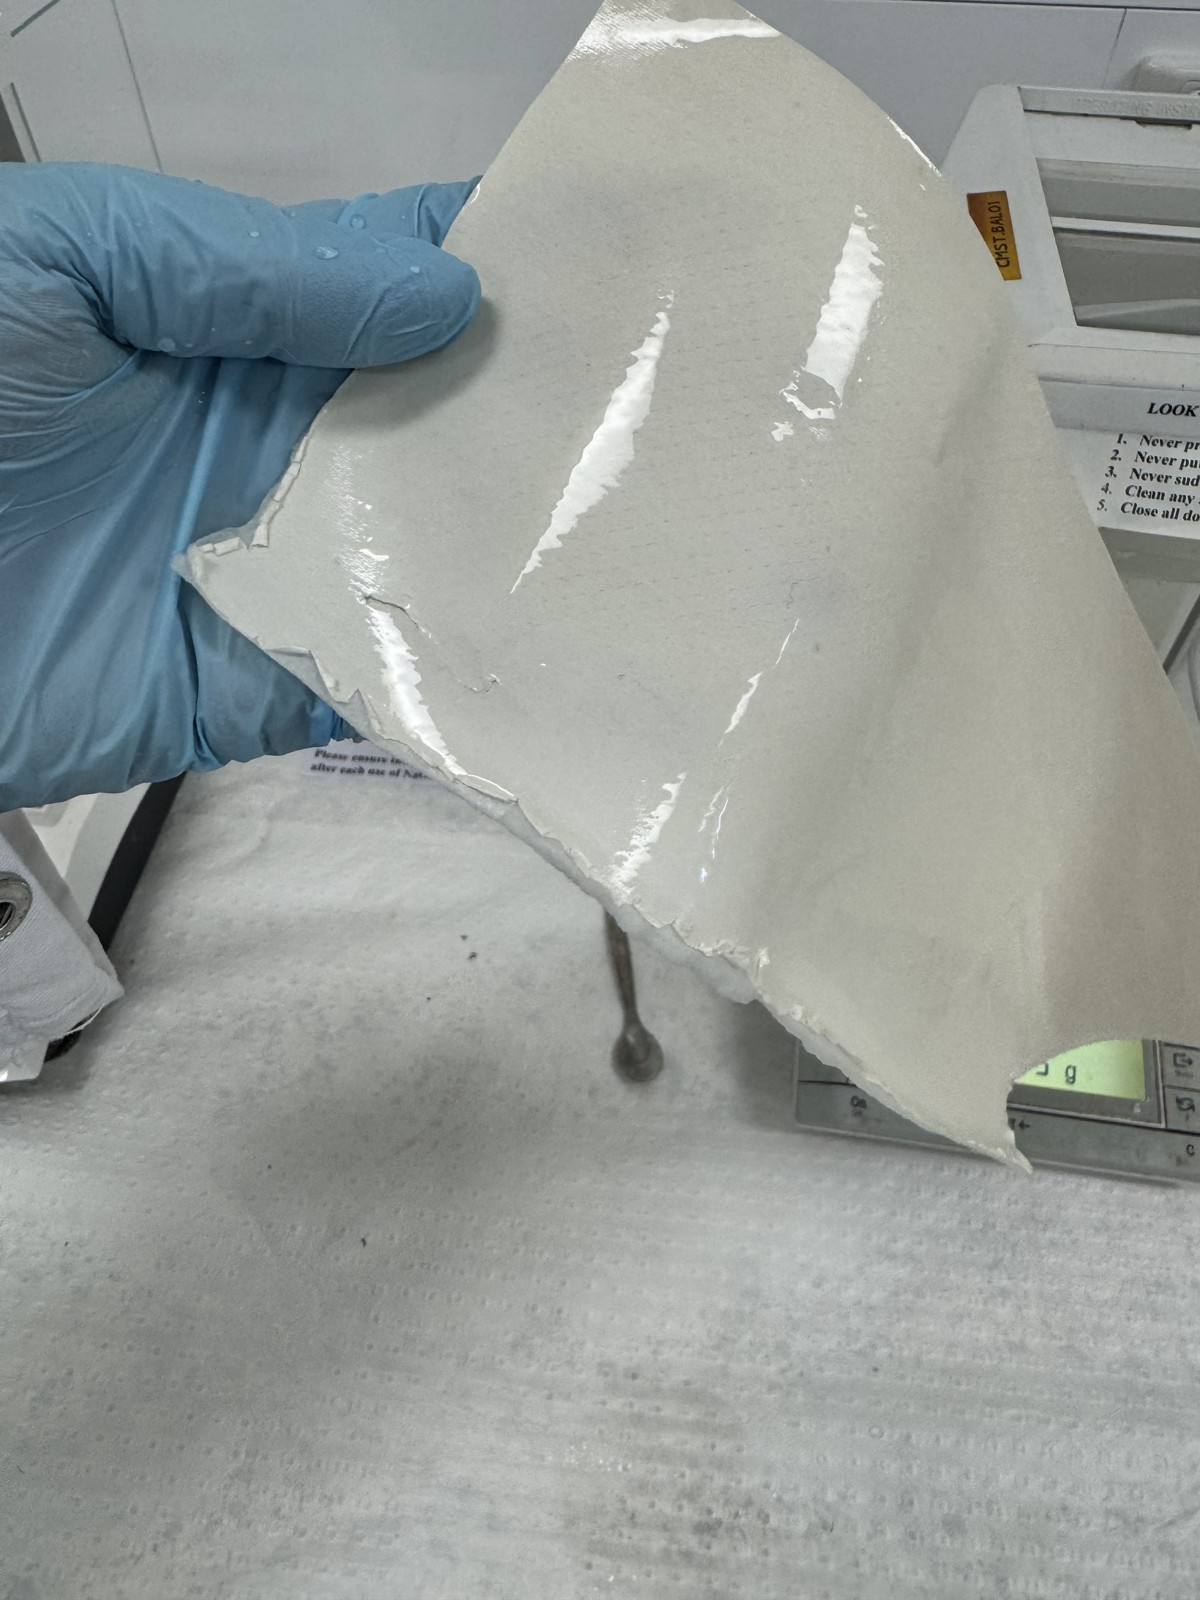
\includegraphics[height=6.5cm]{figures/Cleaned/4297B_delam_whole}\\
    \small (a)
  \end{minipage}\hfill
  \begin{minipage}[b]{0.6\linewidth}
    \centering
    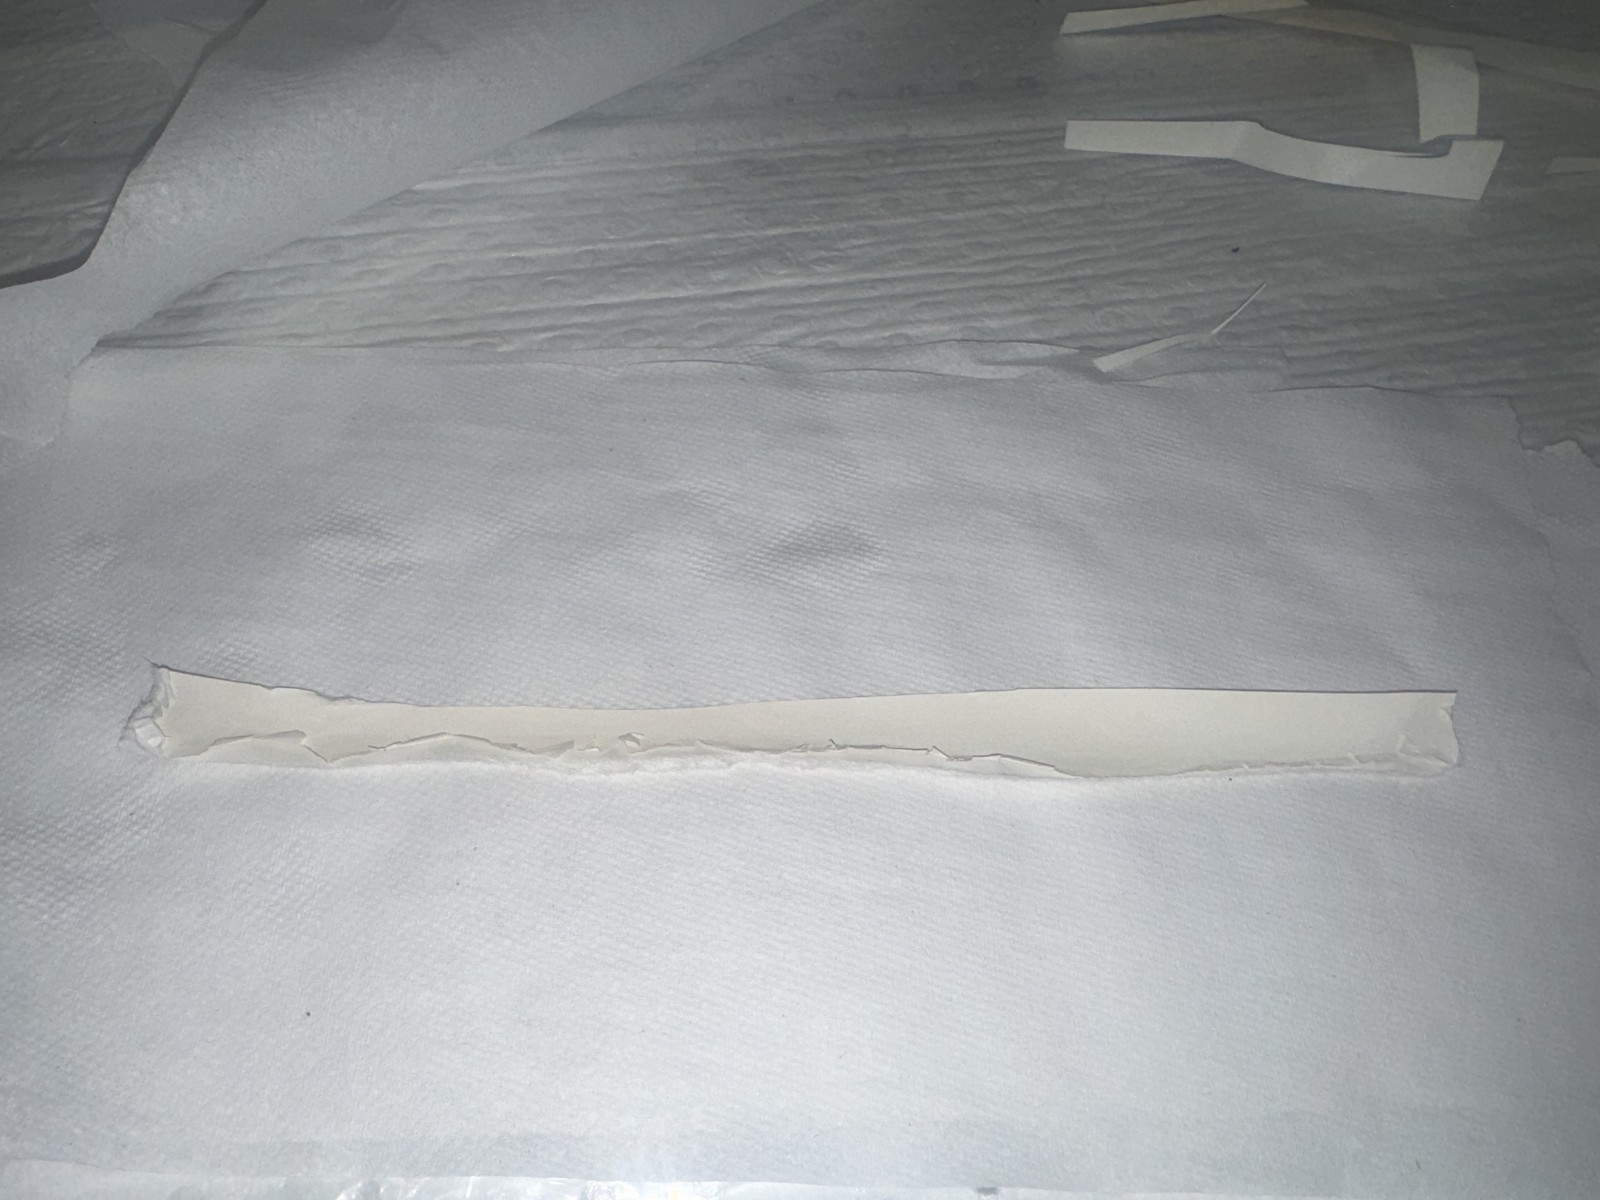
\includegraphics[height=6.5cm]{figures/Cleaned/4297B_delam_strip}\\
    \small (b)
  \end{minipage}
  \caption{Edge delamination of mine-site membrane 4297B after the base clean.}
  \label{fig:4297B-delam}
\end{figure}

\subsection{Performance after cleaning}
\label{sec:res-cleaning-perf}

Table~\ref{tab:clean-compare} shows the flux, PWP and NaCl rejection of the cleaned coupons. As-received values are included for reference and comparison.
\begin{table}[htbp]
  \centering
  \caption{As-received versus cleaned coupons (no IP). Mean $\pm$ SD across coupons; change with Welch's $t$-test $p$-value.}
  \label{tab:clean-compare}
  \small
  \begin{tabular}{llcccc}
    \toprule
    Membrane & Condition & Flux (\unit{LMH}) & PWP (\unit{LMH.bar^{-1}}) & Rejection (\%) & $n$ \\
    \midrule
    4238A & As-received & $1.23 \pm 0.27$ & $0.082 \pm 0.018$ & $78.1 \pm 2.8$ & 2 \\
          & Commercial clean & $2.81 \pm 1.02$ & $0.198 \pm 0.072$ & $86.9 \pm 9.2$ & 2 \\
          & \textbf{Change (\textit{p})} & \textbf{+129\% (0.26)} & \textbf{+142\% (0.25)} & \textbf{+8.8\,pp (0.39)} & \\
    \midrule
    4238C & As-received & $3.21 \pm 0.32$ & $0.208 \pm 0.011$ & $76.6 \pm 3.1$ & 4 \\
          & Extensive clean, all & $4.55 \pm 4.42$ & $0.295 \pm 0.290$ & $79.7 \pm 9.7$ & 7 \\
          & \textbf{Change (\textit{p})} & \textbf{+42\% (0.45)} & \textbf{+42\% (0.46)} & \textbf{+3.1\,pp (0.46)} & \\
          & Extensive clean, excl.\ C5--C6 & $2.04 \pm 1.16$ & $0.130 \pm 0.077$ & $84.3 \pm 6.9$ & 5 \\
          & \textbf{Change (\textit{p})} & \textbf{\textminus 36\% (0.088)} & \textbf{\textminus 37\% (0.086)} & \textbf{+7.7\,pp (0.069)} & \\
    \midrule
    4297B & As-received & $5.22 \pm 1.00$ & $0.330 \pm 0.062$ & $81.9 \pm 8.6$ & 4 \\
          & Extensive clean & $5.60 \pm 1.41$ & $0.359 \pm 0.073$ & $80.5 \pm 11.6$ & 6 \\
          & \textbf{Change (\textit{p})} & \textbf{+7\% (0.64)} & \textbf{+9\% (0.52)} & \textbf{\textminus 1.4\,pp (0.83)} & \\
    \bottomrule
  \end{tabular}
  \par\smallskip
    \footnotesize Flux and PWP at \qtyrange{14}{16}{bar}; rejection with $\sim$\qty{2000}{\milli\gram\per\litre} NaCl. \\95\% confidence intervals of the change: 4238C (excl.\ C5--C6) PWP \qtyrange{-0.172}{0.017}{LMH.bar^{-1}}, rejection \qtyrange{-0.8}{16.3}{pp}; 4297B PWP \qtyrange{-0.072}{0.131}{LMH.bar^{-1}}, rejection \qtyrange{-16.2}{13.3}{pp}.
\end{table}

For 4297B, flux was fairly consistent across the six cleaned coupons, but rejection ranged from \qtyrange{64.2}{91.2}{\percent}, mainly because of two low-rejection coupons. The 4238C coupons varied far more (Table~\ref{tab:clean-desal-coupons}). C5 and C6 had about five times the flux of the others and the lowest rejection. Repeat readings on each coupon agreed within \qty{0.34}{LMH}, so this is not measurement error, and a generalised extreme studentized deviate (ESD) test identified both as outliers (Appendix~\ref{app:outliers}). The high flux and low rejection matched the uneven PA damage seen in the dye test (Figure~\ref{fig:dye_test_full}). They were excluded from the cleaned baseline. 



\begin{table}[htbp]
  \centering
  \caption{Performance of individual extensive clean 4238C (desal) coupons.
  Calculated as the average of repeat readings.}
  \label{tab:clean-desal-coupons}
  \begin{tabular}{lcccc}
    \toprule
    Coupon & $\Delta P$ (\unit{bar}) & Flux (\unit{LMH}) & PWP (\unit{LMH.bar^{-1}}) & NaCl rejection (\%) \\
    \midrule
    C1 & 15.9 & 1.91 & 0.120 & 77.5 \\
    C2 & 15.9 & 2.11 & 0.133 & 78.7 \\
    C3 & 15.8 & 1.65 & 0.105 & 93.2 \\
    C4 & 15.8 & 0.67 & 0.042 & 89.9 \\
    \textbf{C5} & 15.3 & \textbf{9.86} & \textbf{0.644} & \textbf{69.2} \\
    \textbf{C6} & 15.3 & \textbf{11.76} & \textbf{0.768} & \textbf{67.1} \\
    C7 & 15.3 & 3.86 & 0.253 & 82.4 \\
    \midrule
    All coupons ($n = 7$)     & & $4.55 \pm 4.42$ & $0.30 \pm 0.29$ & $79.7 \pm 9.7$ \\
    Excl.\ C5--C6 ($n = 5$)   & & $2.04 \pm 1.16$ & $0.13 \pm 0.08$ & $84.3 \pm 6.9$ \\
    \bottomrule
  \end{tabular}
\end{table}

\subsection{Comparison with the as-received membranes}
 \label{sec:res-cleaning-compare}
No cleaning condition changed PWP or rejection significantly (based on Welch's \textit{t}-test, \textit{p}<0.05). However with such few coupons and wide spread of data, only a very large change would show significant change, so this does not mean cleaning had zero effect. 

\paragraph{4238A (Commercial clean).}
The commercial clean gave the largest changes, with PWP rising by \qty{142}{\percent} and rejection by \qty{8.8}{pp}. Removing foulants would raise both, since it lowers hydraulic resistance and reduces cake-enhanced concentration polarisation \citep{elimelech2005chemical}. Hwowever, the two cleaned coupons varied alot (C1: \qty{0.147}{LMH.bar^{-1}}, \qty{93.4}{\percent}; C2: \qty{0.249}{LMH.bar^{-1}}, \qty{80.4}{\percent}). Each coupon was also tested in a single run so the improvement is indicative only.

\paragraph{4238C (Extensive clean).}
Excluding C5 and C6, PWP fell by \qty{37}{\percent}, and rejection rose by \qty{7.7}{pp}, both close to but not reaching significance (\textit{p} = 0.086 and 0.069). A fall in PWP is not expected from removing foulants, and little foulants was detected in autopsy (Section~\ref{sec:res-fouling-4238C}). Acid tightening of the PA layer may contribute, since acid was the final cleaning step (Section~\ref{sec:lit-cleaning}), but the reported effect of around \qty{10}{\percent} is far smaller than \qty{37}{\percent}. Coupon variation is more likely the cause for this difference \citep{tu2015chemical}. The as-received coupons were consistent with each other, but the cleaned coupons varied 6x in PWP (Table~\ref{tab:clean-desal-coupons}), and C3 and C4, with the highest rejection, probably came from less damaged parts of an unevenly damaged sheet. Cleaning did not improve 4238C, as expected for a membrane that mainly has PA damage. 

\paragraph{4297B (Extensive clean).}
The extensive clean made the smallest difference of the three membranes (PWP \qty{+9}{\percent}, rejection \qty{+1.4}{pp}). This agrees with the autopsy, which did not find much foulants that could be removed with acid and caustic cleans. The change is also similar in size to the effect of cleaning chemicals alone on a clean membrane \citep{tu2015chemical}. Two coupons (C4 and C5) also had higher PWP and lower rejection than the rest, but were not identified as outliers. Excluding them does not change the conclusion for the effects of cleaning (Appendix~\ref{app:outliers}).

\paragraph{Summary.}
Neither cleaning protocol significantly changed PWP or rejection. Because the baseline did not change significantly, changes after IP can be attributed mainly to the new PA layer.


%-------------------––––Next Section-----------------%
\section{Regeneration by IP}
\label{sec:res-ip}
%PWP and rejection for no clean and extensive clean + IP compared with same coupons before


\subsection{Performance after IP}
\label{sec:res-ip-perf}
% Scatter plot: EoLm cleaned and regenerated coupons against new commercial RO and literature NF/UF. 
Table~\ref{tab:ip-results} compares the IP coupons with the as-recieved and cleaned coupons of each membrane. If IP had formed a new selective PA layer, two changes would be expected. First, PWP would fall, as new layer adds a resistance in series with existing membrane. Rejection would also rise, because salt would have to pass through the new layer as well old. 

Because observed rejection depends on water flux as well as on the membrane, PWP and rejection on their own can be misleading when flux changes by many orders of magnitude. The salt permeability coefficient $B$ (Equation~\ref{eq:b-methods}) and the selectivity $A/B$ were therefore also calculated for each coupon (Table~\ref{tab:ip-B}).

\begin{table}[htbp]
  \centering
  \caption{Performance before and after IP. Mean $\pm$ SD across coupons; change with Welch's $t$-test $p$-value.}
  \label{tab:ip-results}
  \small
  \setlength{\tabcolsep}{4pt}
  \begin{tabular}{llcccc}
    \toprule
    Membrane & Condition & Flux (\unit{LMH}) & PWP (\unit{LMH.bar^{-1}}) & Rejection (\%) & $n$ \\
    \midrule
    4238C & As received                     & $3.21 \pm 0.32$ & $0.208 \pm 0.011$ & $76.6 \pm 3.1$ & 4 \\
          & Extensive clean (excl.\ C5--C6) & $2.04 \pm 1.16$ & $0.130 \pm 0.077$ & $84.3 \pm 6.9$ & 5 \\
          & Extensive clean + IP            & $0.35 \pm 0.20$ & $0.023 \pm 0.013$ & $76.2 \pm 7.9$ & 4 \\
          & \textbf{Change vs as received (\textit{p})} & \textbf{\textminus 89\% (<0.001)} & \textbf{\textminus 89\% (<0.001)} & \textbf{\textminus 0.4\,pp (0.92)} & \\
          & \textit{Change vs cleaned (\textit{p})}     & \textit{\textminus 83\% (0.030)}  & \textit{\textminus 82\% (0.034)}  & \textit{\textminus 8.2\,pp (0.15)} & \\
          & No clean + IP  & $0.95 \pm 0.16$ & $0.061 \pm 0.010$ & $86.9 \pm 0.5$ & 2 \\
          & \textbf{Change vs as received (\textit{p})} & \textbf{\textminus 70\% (<0.001)} & \textbf{\textminus 71\% (0.003)} & \textbf{+10.3\,pp (0.006)} & \\
    \midrule
    4297B & As received                     & $5.22 \pm 1.00$ & $0.330 \pm 0.062$ & $81.9 \pm 8.6$  & 4 \\
          & Extensive clean                 & $5.60 \pm 1.41$ & $0.359 \pm 0.073$ & $80.5 \pm 11.6$ & 6 \\
          & Extensive clean + IP            & $0.69 \pm 0.19$ & $0.046 \pm 0.012$ & $80.5 \pm 11.1$ & 2 \\
          & \textbf{Change vs as received (\textit{p})} & \textbf{\textminus 87\% (0.002)} & \textbf{\textminus 86\% (0.002)} & \textbf{\textminus 1.4\,pp (0.89)} & \\
          & \textit{Change vs cleaned (\textit{p})}     & \textit{\textminus 88\% (<0.001)} & \textit{\textminus 87\% (<0.001)} & \textit{0.0\,pp (1.00)} & \\
    \midrule
    4238A & As received                     & $1.23 \pm 0.27$ & $0.082 \pm 0.018$ & $78.1 \pm 2.8$ & 2 \\
          & Commercial clean                & $2.81 \pm 1.02$ & $0.198 \pm 0.072$ & $86.9 \pm 9.2$ & 2 \\
          & Commercial clean + IP           & $1.32 \pm 0.17$ & $0.093 \pm 0.012$ & $87.1 \pm 0.7$ & 2 \\
          & \textbf{Change vs as received (\textit{p})} & \textbf{+7\% (0.73)} & \textbf{+14\% (0.54)} & \textbf{+9.1\,pp (0.12)} & \\
          & \textit{Change vs cleaned (\textit{p})}     & \textit{\textminus 53\% (0.28)} & \textit{\textminus 53\% (0.28)} & \textit{+0.2\,pp (0.98)} & \\
          & No clean + IP                   & $2.00 \pm 0.44$ & $0.138 \pm 0.030$ & $85.6 \pm 0.8$ & 2 \\
          & \textbf{Change vs as received (\textit{p})} & \textbf{+63\% (0.20)} & \textbf{+68\% (0.19)} & \textbf{+7.5\,pp (0.14)} & \\
    \bottomrule
  \end{tabular}
  \par\smallskip
  \footnotesize Bold: net effect of regeneration (vs as received). Italic: effect of the IP step alone (vs cleaned). Flux and PWP at \qtyrange{14}{16}{bar}; rejection with $\sim$\qty{2000}{\milli\gram\per\litre} NaCl (\qtyrange{3560}{4300}{\micro\siemens\per\centi\metre}).
\end{table}

\paragraph{Desal-site first-pass membrane 4238A}
4238A showed did not show a large PWP drop. After the commercial clean and IP, PWP was \qty{0.093}{} $\pm$ \qty{0.012}{LMH.bar^{-1}}, \qty{14}{\percent} above the as received membranes (p = 0.54) and \qty{53}{\percent} below the cleaned coupons (p = 0.28). Rejection was $87.1 \pm \qty{0.7}{\percent}$, essentially the same as the cleaned value ($+0.2$ pp, $p = 0.98$). Without a clean, IP gave $0.138 \pm \qty{0.030}{LMH.bar^{-1}}$ and $85.6 \pm \qty{0.8}{\percent}$. Neither results differs significantly from as-received. The rejection of both IP membranes (\qtyrange{85.6}{87.1}{\percent}) was close to that of the cleaned coupons. 4238A was intact and within specification, so there was little for IP to repair. 

\paragraph{Desal-site second-pass membrane 4238C}
IP gave a large and consistent drop in PWP on 4238C. With the extensive clean before IP, PWP fell from $0.208 \pm 0.011$ to $0.023 \pm \qty{0.013}{LMH.bar^{-1}}$ (\qty{-89}{\percent}, $p < 0.001$). IP step itself reduced PWP by \qty{82}{\percent} ($p = 0.034$). Without cleaning, IP reduced PWP by \qty{71}{\percent} to $0.061 \pm \qty{0.010}{LMH.bar^{-1}}$ ($p = 0.003$). Both IP added a huge hydraulic resistance to the membrane. 

The rejection results did not match expectation. With extensive clean, rejection after IP was $76.2 \pm \qty{7.9}{\percent}$, which is the same as the as-received value ($-0.4$ pp, $p =0.92$), and \qty{8.2}{pp} below the cleaned coupons (p = 0.15). The no-clean + IP was the only one that raised rejection, by \qty{10.3}{pp} to $86.9 \pm \qty{0.5}{\percent}$ ($p = 0.006$). It is also the only significant rejection change in the study. The two no-clean + IP coupons agree closely but with only two coupons, and the result coming from campaign 1 (before stricter controls and better methodology), so these results should be treated as indicative. \flag{DO THIS} Section~\ref{sec:res-cleaning-effect} discusses why the uncleaned support gave a better result than the cleaned one. 

\paragraph{Mine-site membrane 4297B}
4297B responded the same way as the cleaned 4238C membrane. After extensive clean and IP, PWP fell by \qty{86}{\percent} to $0.046 \pm \qty{0.012}{LMH.bar^{-1}}$ (p = 0.002) or by \qty{87}{\percent} compared with the cleaned coupons ($p < 0.001$). Rejection did not change at all, testing at $80.5 \pm \qty{11.1}{\percent}$ after IP against $80.5 \pm \qty{11.6}{\percent}$ after cleaning. Only two coupons were tested, and the large SD comes from a wide gap between them (\qty{88.4}{\percent} and \qty{72.6}{\percent}). So while one coupon showed a  \qty{9.3}{pp} decrease in salt rejection, the other coupon showed a \qty{6.5}{pp} increase. 

\subsection{Salt permeability and selectivity}
\label{sec:res-ip-B}
Comparing rejection directly can be misleading when the flux changes so much. If the salt permeability $B$ stays constant, the observed rejection falls when water flux falls, as salt passes through the membrane at the same rate, but there is less water diluting it. In the solution diffusion model, the intrinsic solute rejection (R) is defined as $R = \frac{J_w}{J_w + B}$ \flag{Might need source or derivation https://mcba.co.uk/water-treatment-systems/membrane-transport-solution-diffusion/}. If the as-received 4238C membrane with $B \approx \qty{0.98}{LMH}$ (substituting from results) was run at a post IP flux of \qty{0.35}{LMH}, the rejection would have fallen to about \qty{26}{\percent}. The IP coupons rejected \qty{76}{\percent} at that flux, so the IP layer must have lowered salt permeability substantially. 

Table~\ref{tab:ip-B} gives $B$ (Equation~\ref{eq:b-methods}) and the selectivity $A/B$ for each condition, where $A$ is taken as the PWP.

\begin{table}[htbp]
\centering
\caption{Salt permeability coefficient $B$ and selectivity $A/B$ for each condition. \flag{Currently estimated from mean flux and rejection; replace with per-coupon mean $\pm$ SD.}}
\label{tab:ip-B}
\small
\begin{tabular}{llccc}
    \toprule
    Membrane & Condition & $A$ (\unit{LMH.bar^{-1}}) & $B$ (\unit{LMH}) & $A/B$ (\unit{bar^{-1}}) \\
    \midrule
    4238A & As received & 0.082 & 0.35 & 0.24 \\
    & Commercial clean & 0.198 & 0.42 & 0.47 \\
    & Commercial clean + IP & 0.093 & 0.20 & 0.47 \\
    & No clean + IP & 0.138 & 0.34 & 0.41 \\
    \midrule
    4238C & As received & 0.208 & 0.98 & 0.21 \\
    & Extensive clean (excl.\ C5--C6) & 0.130 & 0.38 & 0.34 \\
    & Extensive clean + IP & 0.023 & 0.11 & 0.21 \\
    & No clean + IP & 0.061 & 0.14 & 0.43 \\
    \midrule
    4297B & As received & 0.330 & 1.15 & 0.29 \\
    & Extensive clean & 0.359 & 1.36 & 0.26 \\
    & Extensive clean + IP & 0.046 & 0.17 & 0.28 \\
    \bottomrule
  \end{tabular}
\end{table}

\iffalse
On 4238A, the commercial clean alone roughly doubled $A/B$ (\qtyrange{0.24}{0.47}{bar^{-1}}). IP lowered both $A$ and $B$ by about half but did not change selectivity further. Without a clean, IP gave a similar $A/B$ of \qty{0.41}{bar^{-1}}.

On 4238C and 4297B, IP in the cleaned arms lowered $B$ by about the same fraction as $A$. On 4238C, $B$ fell by about \qty{89}{\percent} from as-received, matching the \qty{89}{\percent} fall in PWP. On 4297B, $B$ fell by about \qty{88}{\percent} from the cleaned value, against \qty{87}{\percent} for PWP. As a result, $A/B$ was almost unchanged: \qty{0.21}{bar^{-1}} before and after on 4238C, and \qtyrange{0.26}{0.28}{bar^{-1}} on 4297B. The new layer therefore slowed water and salt by about the same amount. It acted as an extra resistance but did not make the membrane more selective. A dense, defect-free PA film in series with the old membrane should lower $B$ much more than $A$ and raise $A/B$ \flag{cite series-resistance/selectivity source}. Unchanged selectivity instead points to a film that is very thin or patchy over the damaged areas, or to salt passing through a route the new layer does not cover.

The second possibility links back to the coupon offset in Section~\ref{sec:res-baseline}. Salt that bypasses the PA, through defects at the cut edge or past the O-ring seal, flows convectively and is not affected by any new layer. When water flux through the membrane falls by an order of magnitude, a fixed leak becomes a much larger share of the permeate and puts a ceiling on observed rejection. The rejection of the cleaned 4238C and 4297B conditions sat in a narrow \qtyrange{76}{84}{\percent} band whatever the PWP, which is consistent with such a ceiling. This study cannot tell the two explanations apart. \flag{Was a blank/sealed coupon or dye test run after IP? If so, cite here.}

The no-clean arm on 4238C was the only IP condition where selectivity clearly increased. $A/B$ roughly doubled, from \qtyrange{0.21}{0.43}{bar^{-1}}, because $B$ fell by \qty{85}{\percent} while PWP fell by only \qty{71}{\percent}.
\fi


\subsection{Surface characterisation}
\label{sec:res-surface}
\paragraph{FTIR.}
ATR-FTIR spectra of the as-received, extensive-clean and extensive clean + IP coupons are shown in Figure~\ref{fig:ftir}. ATR-FTIR also samples below the PA layer, so most of the signal comes from the polysulfone support and looks similar. Changes were judged from the PA band heights relative to the polysulfone band (Table~\ref{tab:ftir_ratios}).

Cleaning did not change the PA bands of 4238C, with all three ratios within \qty{3}{\percent} of the EoL values. On 4297B, the PA bands fell by about \qtyrange{8}{9}{\percent} after cleaning. This may be due to the removal of organic foulants that absorb at similar positions. No foulant bands could be identified on either membrane, as the deposits were light.

After IP, the PA bands of 4238C increased by about \qtyrange{30}{50}{\percent} relative to the support (amide~I from 0.38 to 0.50, amide~II from 0.44 to 0.65), confirming that a new PA layer had formed. On 4297B, the PA bands did not increase after IP, even though its PWP fell by as much as that of 4238C (Section~\ref{sec:res-ip-perf}). This suggests the layer formed on 4297B was too thin or uneven to show in FTIR.

\begin{table}[htbp]
    \centering
    \caption{FTIR absorbance ratios of PA bands to the polysulfone band at \qty{1488}{cm^{-1}} (mean $\pm$ SD of three scans).}
    \label{tab:ftir_ratios}
    \begin{tabular}{llccc}
        \toprule
        Membrane & Condition & Amide I / PSf & Amide II / PSf & N--H/O--H / PSf \\
        \midrule
        4238C & EoL          & $0.38 \pm 0.01$ & $0.44 \pm 0.01$ & $0.11 \pm 0.00$ \\
              & Cleaned      & $0.37 \pm 0.01$ & $0.43 \pm 0.01$ & $0.11 \pm 0.01$ \\
              & Cleaned + IP & $0.50 \pm 0.02$ & $0.65 \pm 0.03$ & $0.15 \pm 0.00$ \\
        \midrule
        4297B & EoL          & $0.32 \pm 0.01$ & $0.37 \pm 0.02$ & $0.11 \pm 0.00$ \\
              & Cleaned      & $0.30 \pm 0.00$ & $0.33 \pm 0.01$ & $0.10 \pm 0.00$ \\
              & Cleaned + IP & $0.29 \pm 0.01$ & $0.33 \pm 0.01$ & $0.09 \pm 0.00$ \\
        \bottomrule
    \end{tabular}
\end{table}

\begin{figure}[htbp]
  \centering
  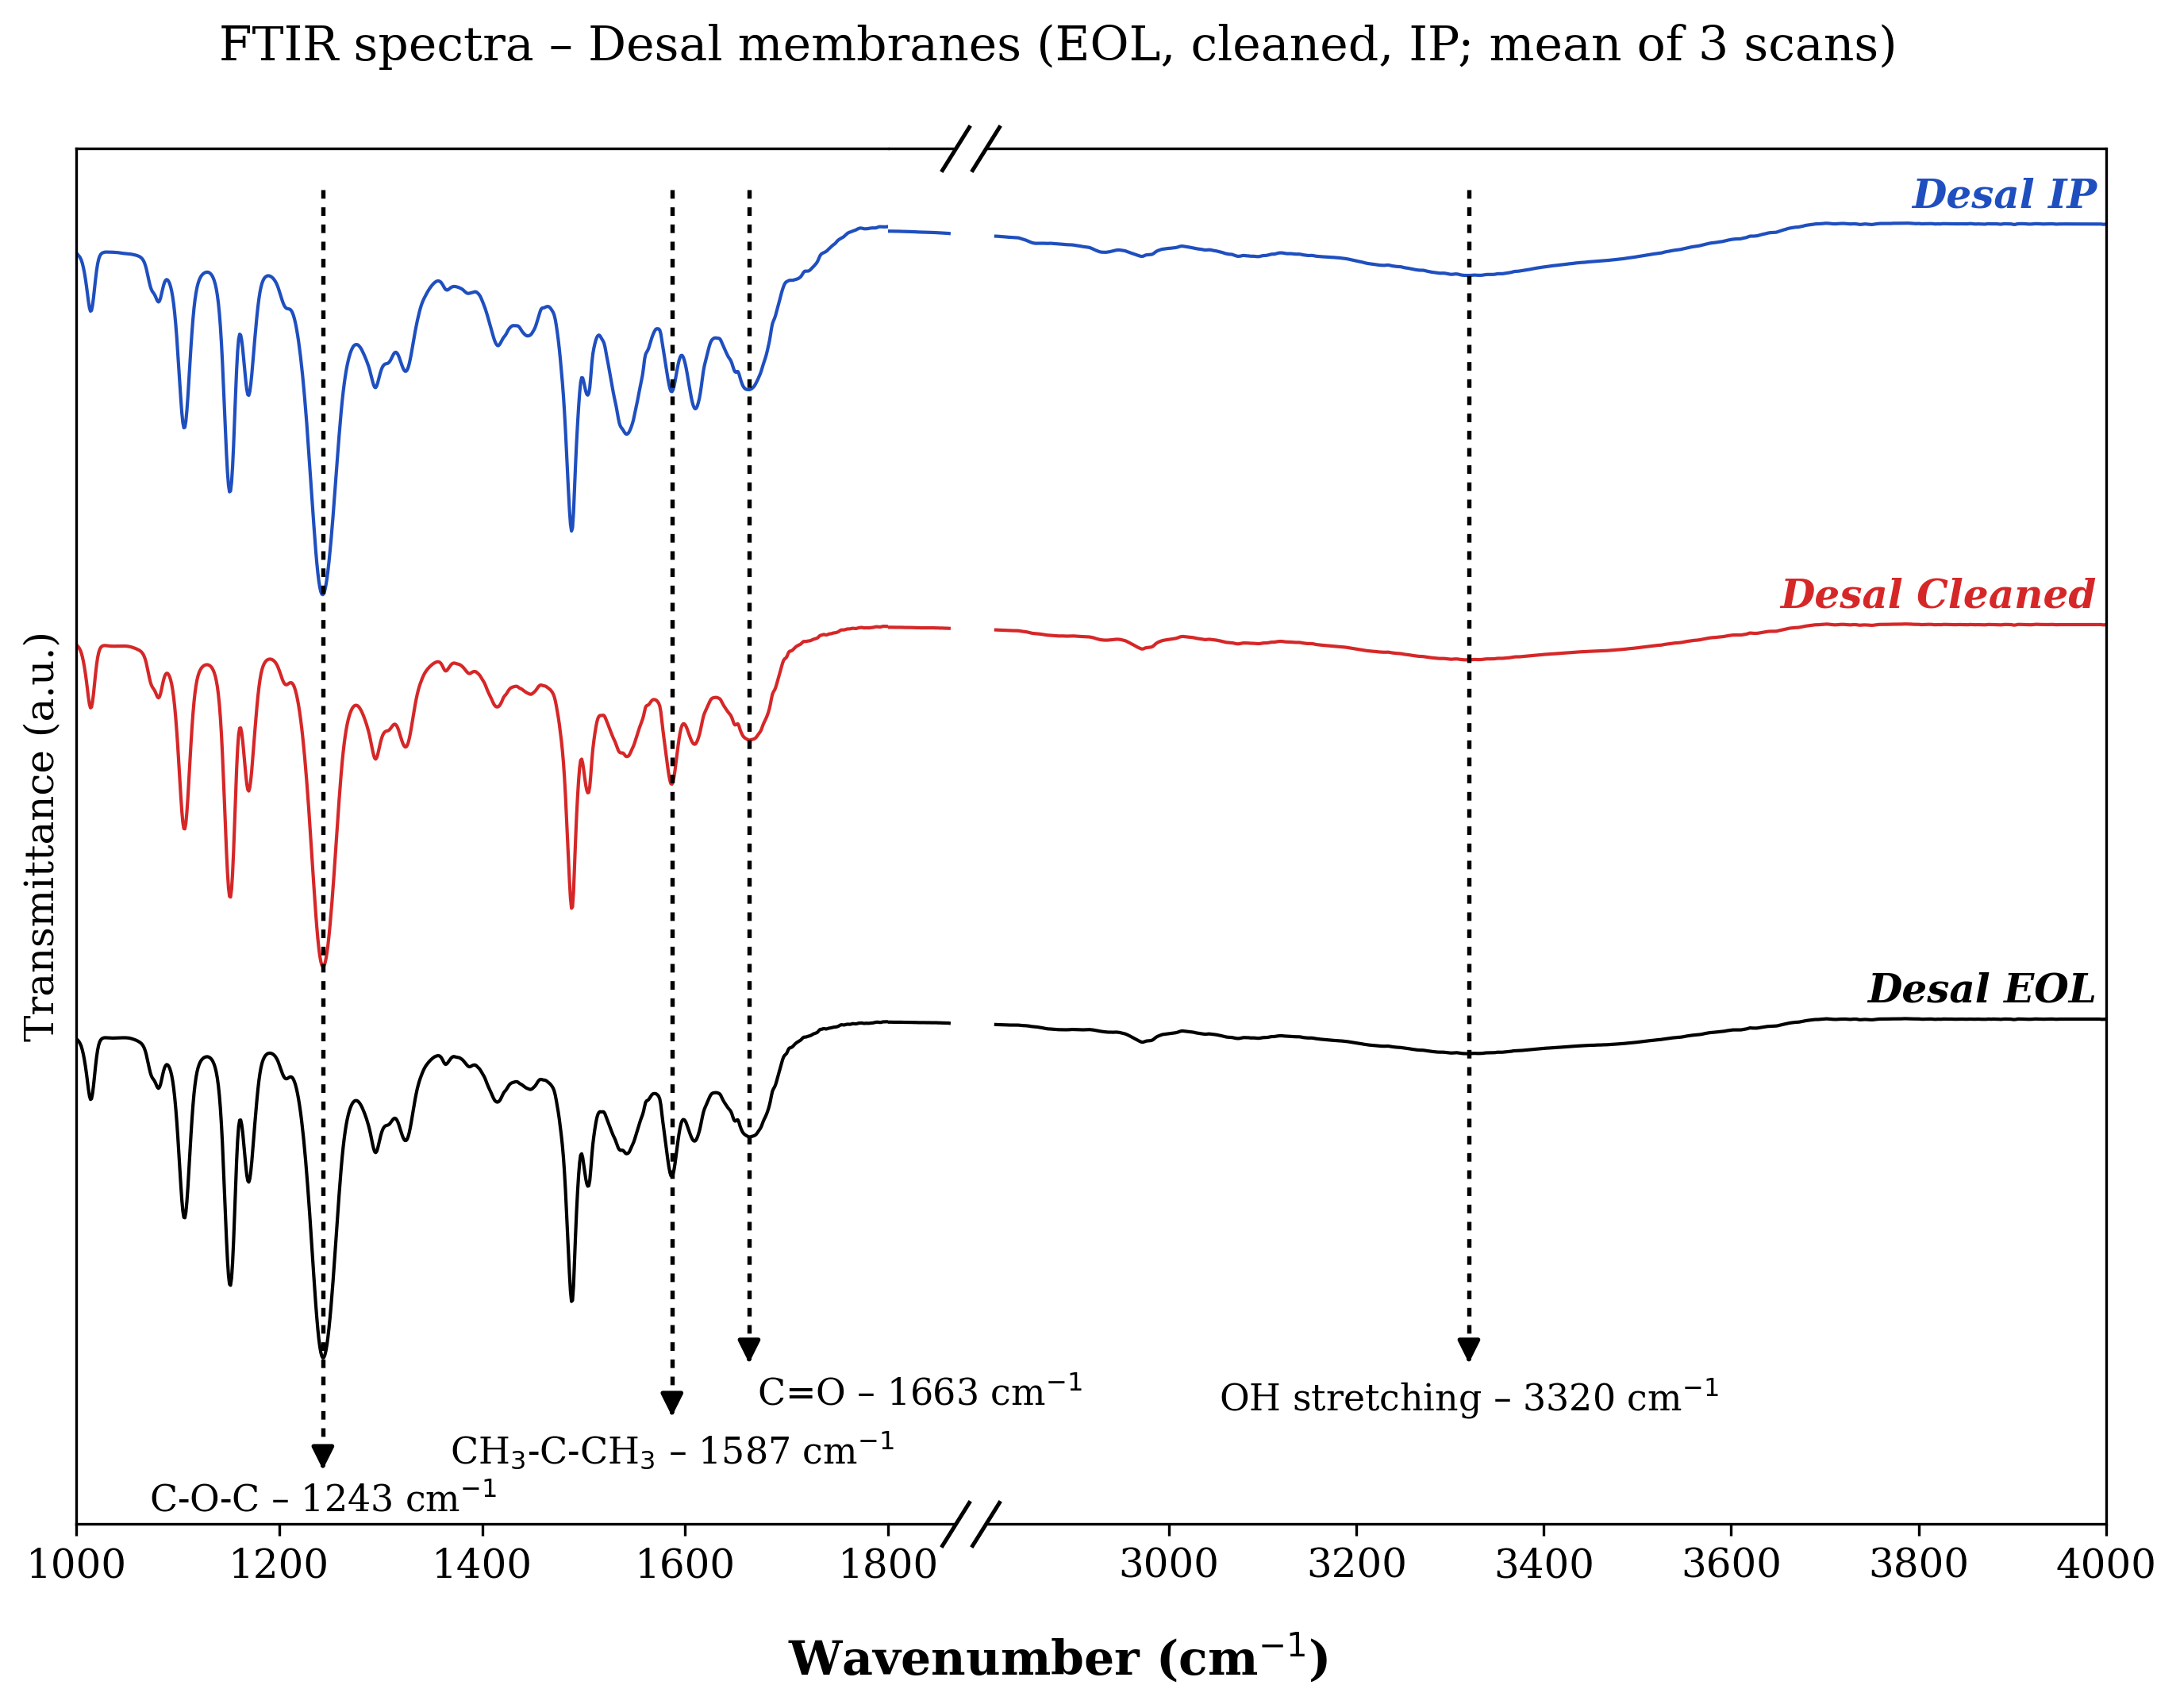
\includegraphics[width=0.6\linewidth]{figures/Analysis/FTIR/FTIR_Desal_stacked}\\
  \small (a) Desal-site membrane 4238C\\[3pt]
  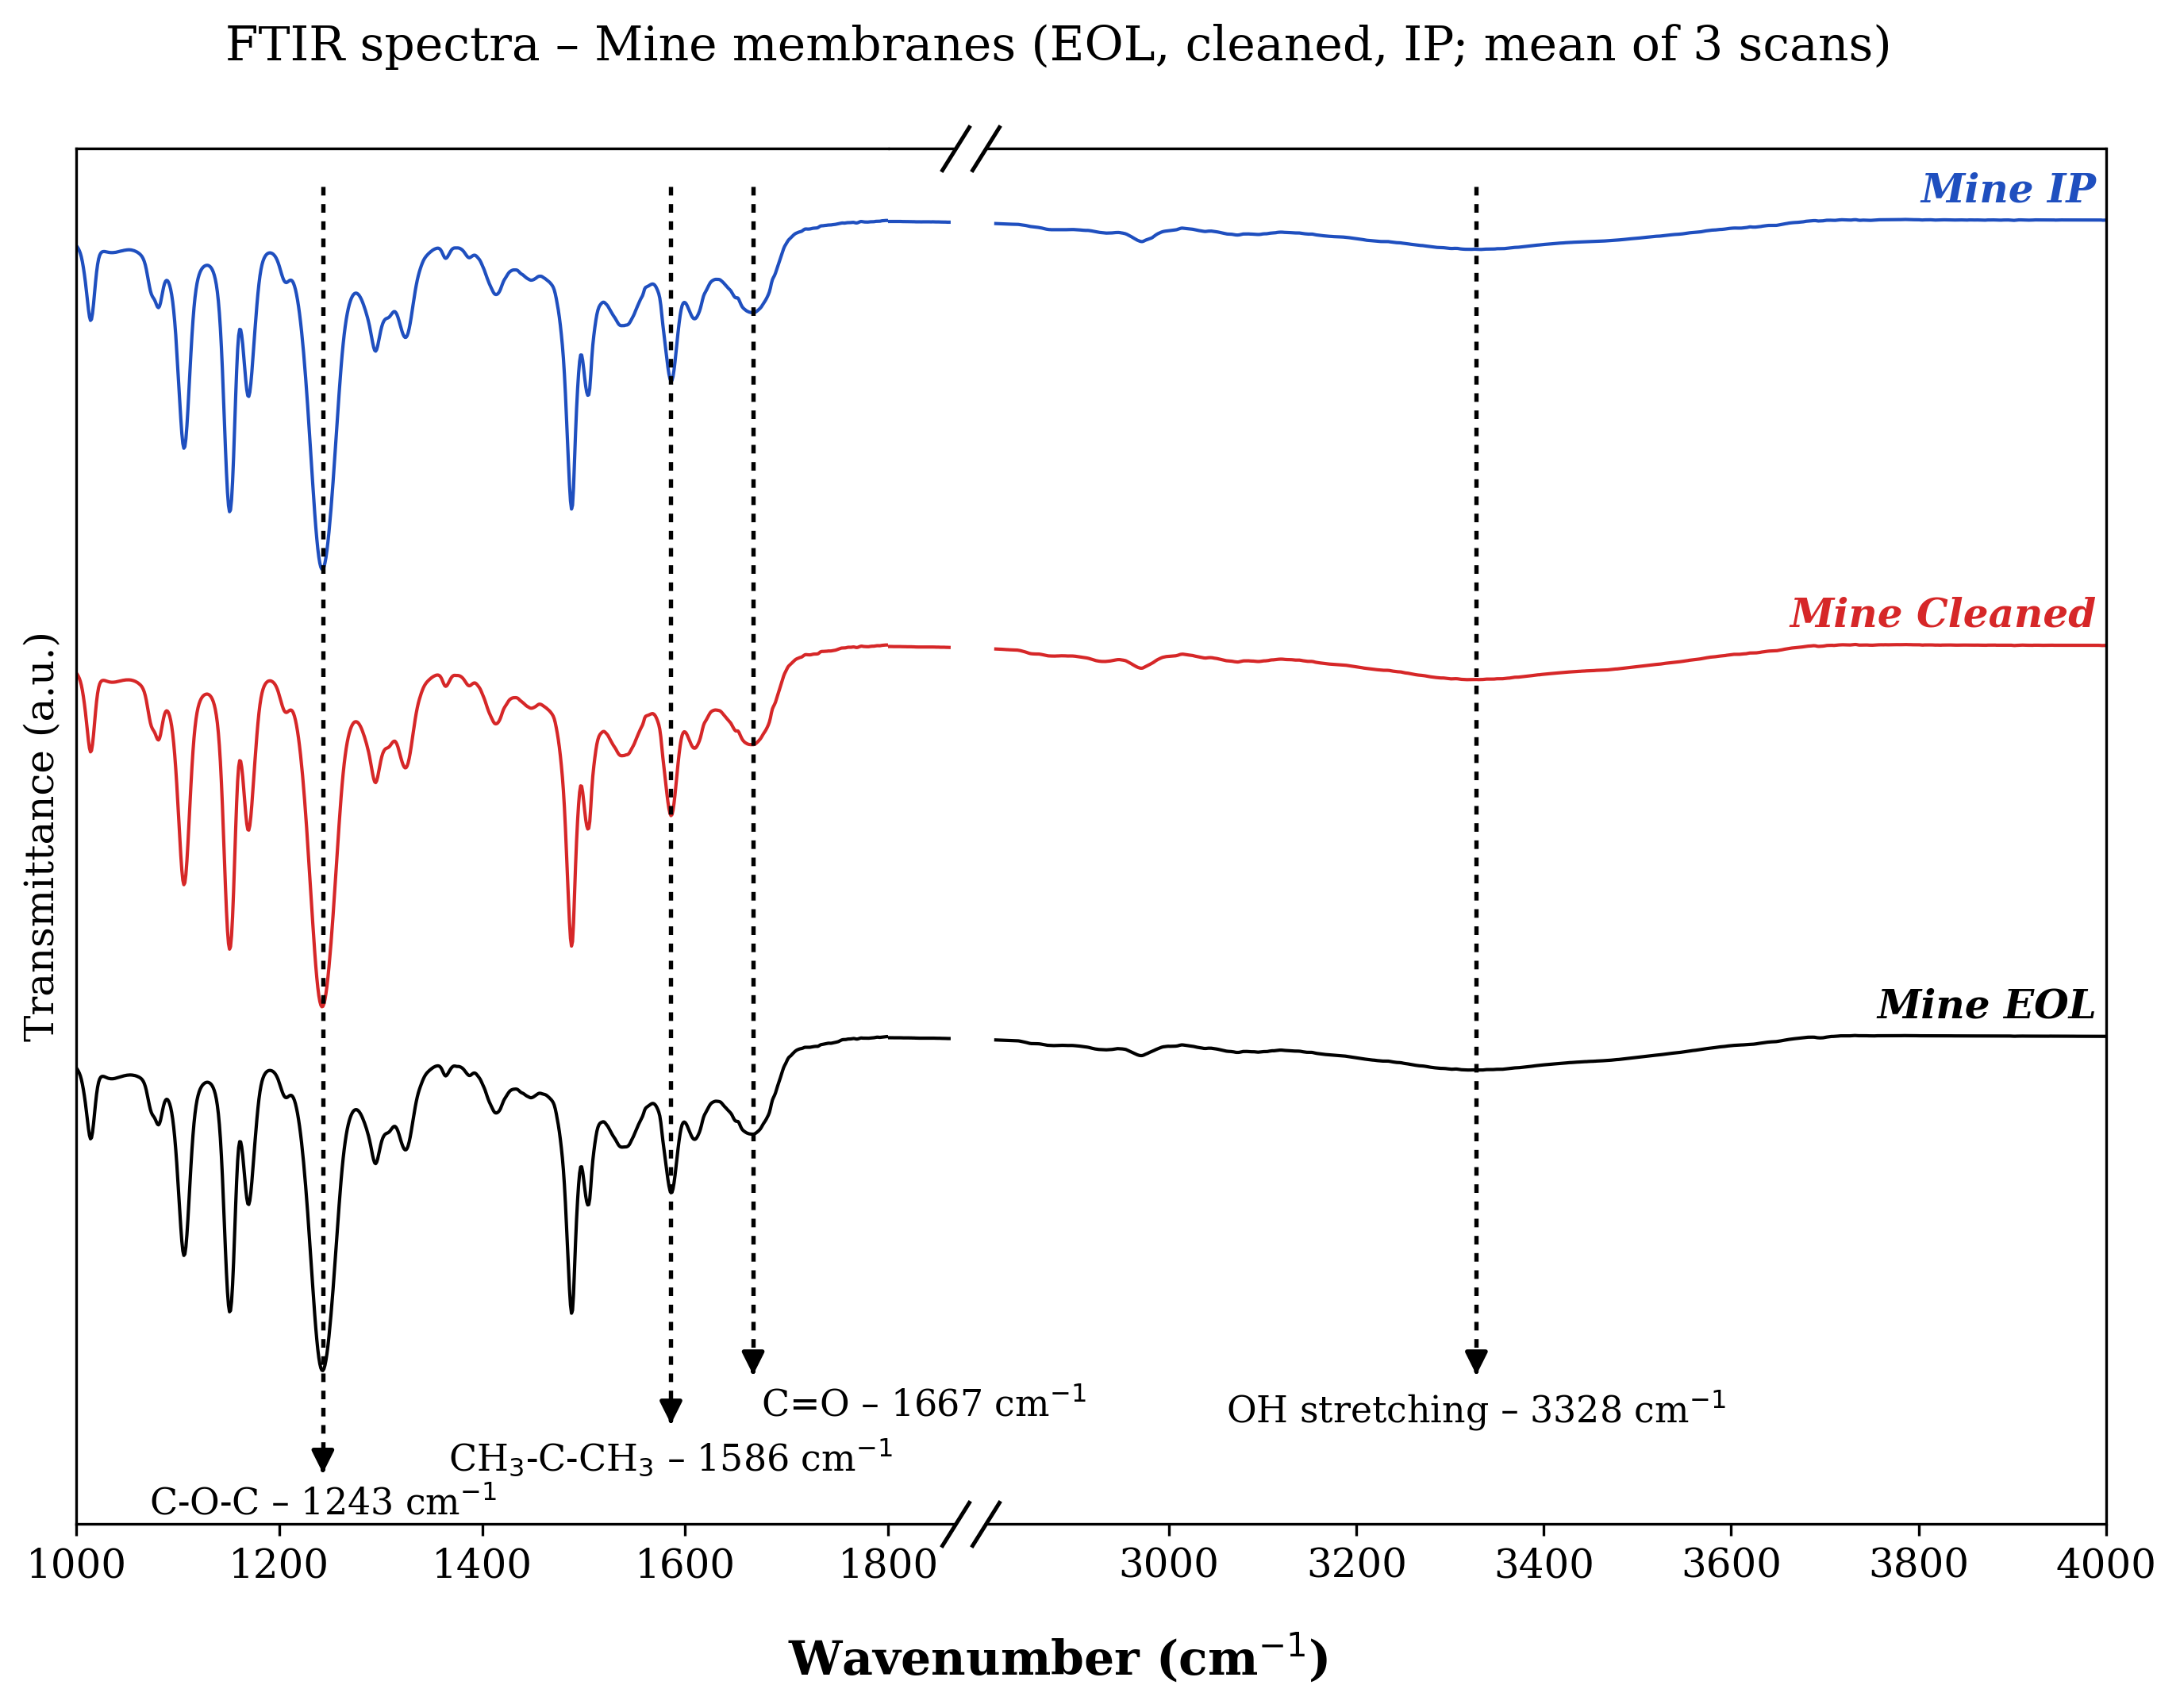
\includegraphics[width=0.6\linewidth]{figures/Analysis/FTIR/FTIR_Mine_stacked}\\
  \small (b) Mine-site membrane 4297B
  \caption{ATR-FTIR spectra of EoL, extensive-clean and extensive-clean + IP coupons of (a) 4238C and (b) 4297B.}
  \label{fig:ftir}
\end{figure}

\paragraph{SEM of 4238C.}
The EoL 4238C surface had a much less dense PA layer, with larger gaps between the PA structures (Figure~\ref{fig:sem_4238C_comparison}a). This is consistent with the PA damage found in the autopsy \citep{MembraneWorks2025Desal} and with the high flux and low rejection pattern on this sample. The cleaned surface showed a normal ridge-and-valley structure though the magnification made this difficult to judge (Figure~\ref{fig:sem_4238C_comparison}b). After IP, the PA was lightly more dense  (Figure~\ref{fig:sem_4238C_comparison}c), which attributed to the drop in PWP.

\begin{figure}[htbp]
\centering
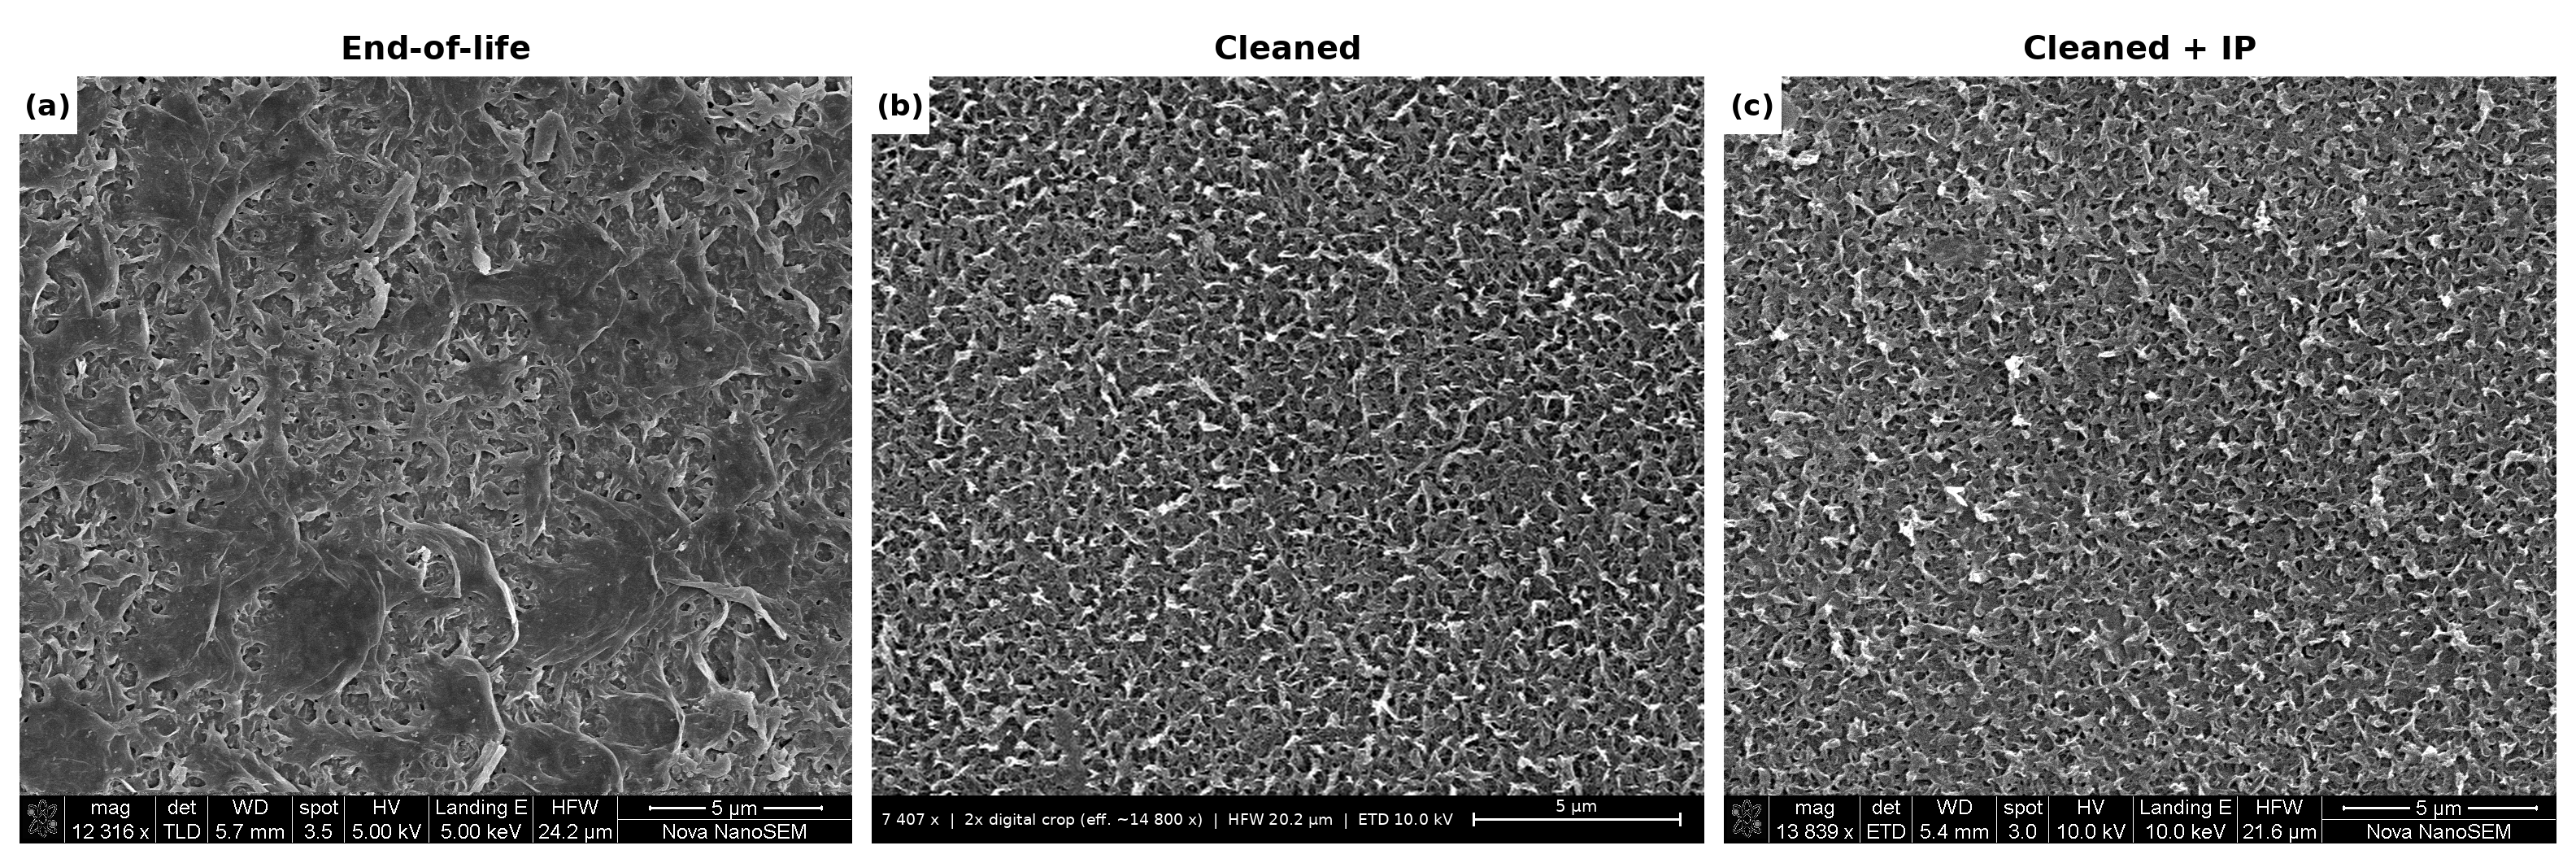
\includegraphics[width=\textwidth]{figures/Analysis/SEM/Fig_4238C_comparison_SEM.png}
\caption{SEM of 4238C (desal-site) surfaces: (a) end-of-life; (b) extensive clean; (c) extensive clean + IP}
\label{fig:sem_4238C_comparison}
\end{figure}

\paragraph{SEM of 4297B.}
The EoL 4297B surface showed a ridge-and-valley PA structure with granular deposits (Figure~\ref{fig:sem_4297B}a). After cleaning, these was little visible change (Figure~\ref{fig:sem_4297B}b). After IP, a much denser, crosslinked structure was visible (Figure~\ref{fig:sem_4297B}c). The granular deposit were still present on the clean + IP surface. This is consistent with the expected cleaning response, where the iron oxide and silica deposits were not expected to be removed during cleaning (Section~\ref{sec:res-fouling})\citep{MembraneWorks2026Mine}. The new layer on 4297B waas less uniform and flat than on 4238C. This agrees with residual foulants interfering with layer formation. 

\begin{figure}[htbp]
\centering
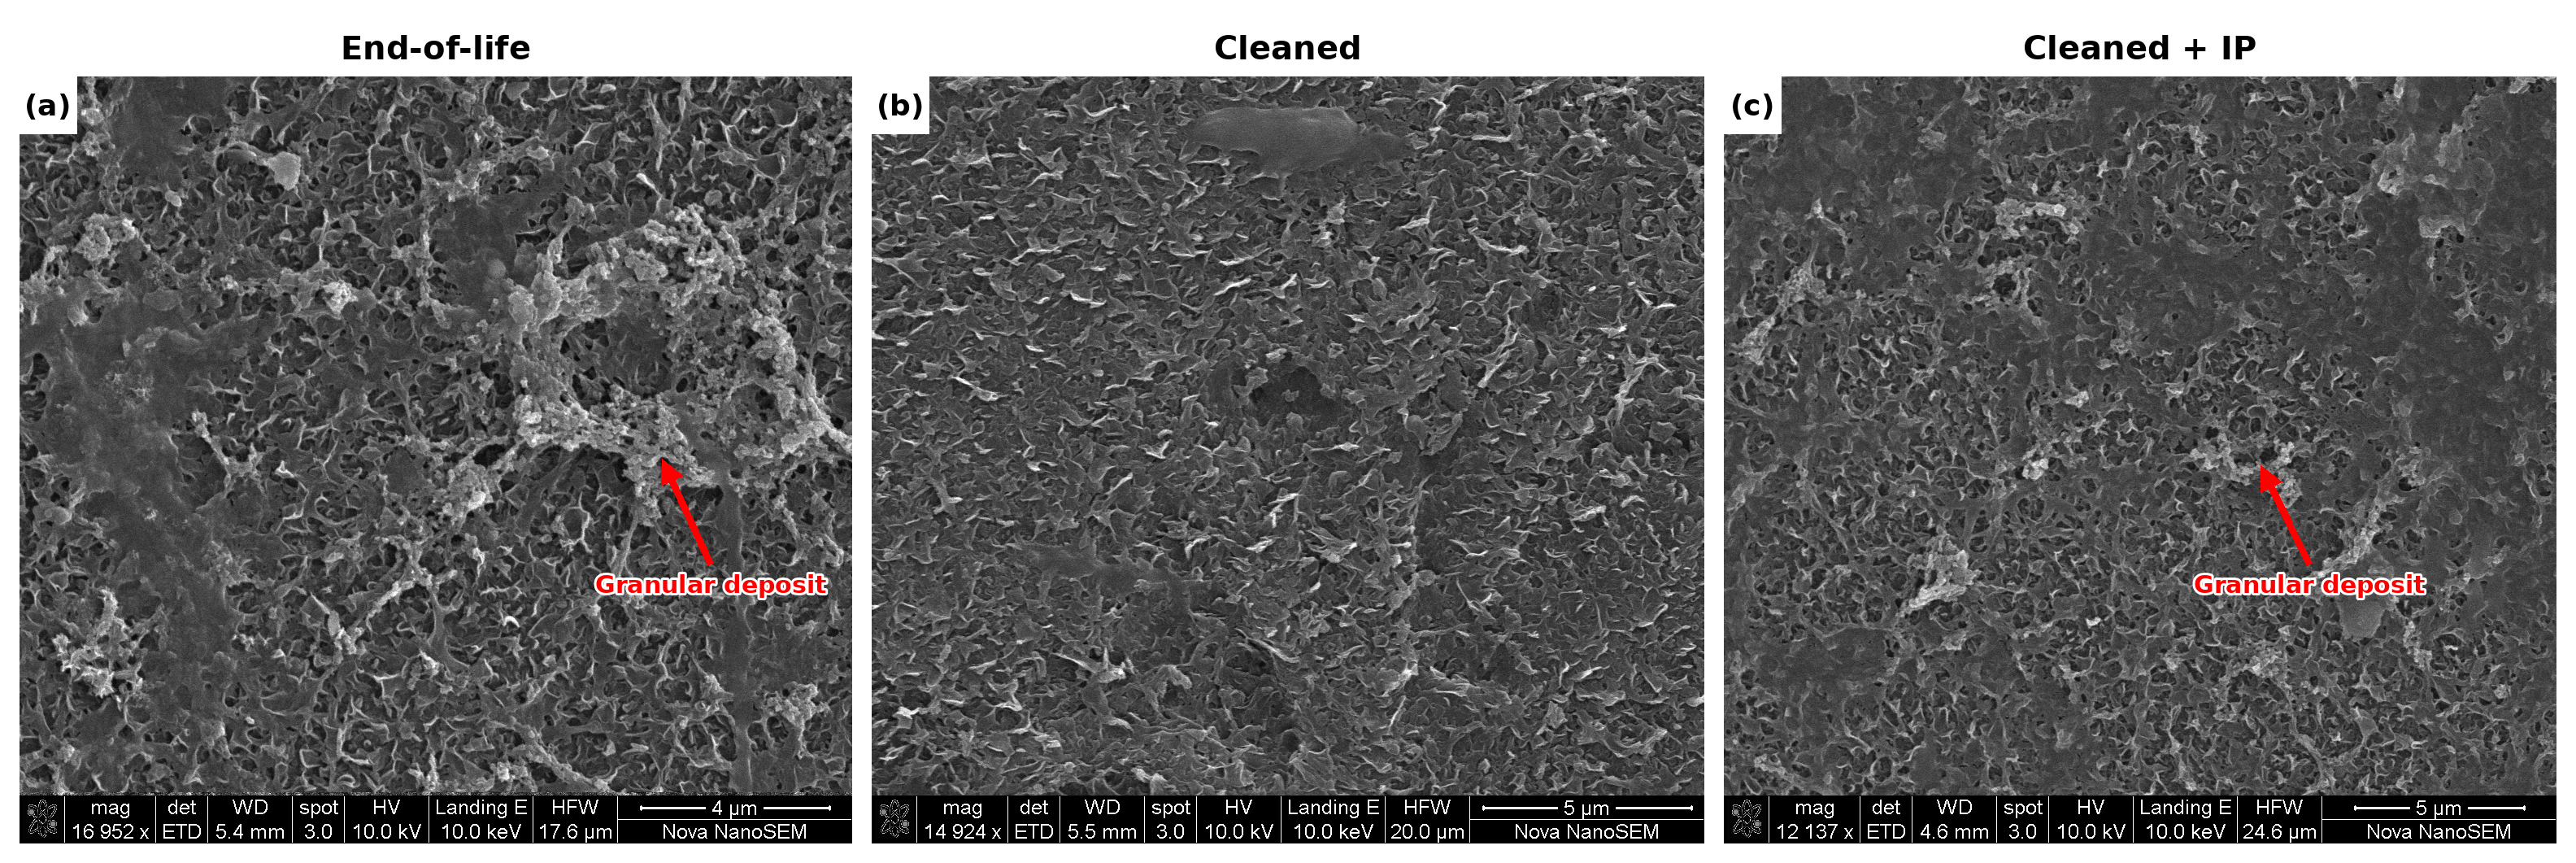
\includegraphics[width=\textwidth]{figures/Analysis/SEM/Fig_4297B_SEM.png}
\caption{SEM micrographs of 4297B (mine-site) surfaces: (a) end-of-life; (b) extensive clean; (c) extensive clean + IP.}
\label{fig:sem_4297B}
\end{figure}

\paragraph{Summary.}
Cleaning did not change the PA layer of either membrane significantly, and granular deposits on 4297B remained after cleaning. IP formed a new, denser PA layer on both membrane, but on 4238C it was uniform and clearly detected by FTIR, and on 4297B it was less uniform and not detected. 


%---------Discussion---------------%
\section{Effect of cleaning on regeneration 500-600 words}
\label{sec:res-cleaning-effect}
Answers: whether the support layer must be cleaned before IP for regeneration to work at all. 

\begin{itemize}
  \item no clean versus extensive clean, for both membranes.
  \item an uncleaned support layer should yield a defective film --- high permeability, low rejection, wide replicate scatter.
  \item does the cleaned arm reach commercial RO territory, or only improve on the uncleaned one? 
  \item Distinguish a real effect from replicate scatter; state  limits of what replicate can support.
  \item If the cleaned arm does not deliver the expected permeability drop and rejection gain, interpret  against the five mechanisms in Section~\ref{sec:fouling-ip}
\end{itemize}
\citet{Singh2006} \flag{showed reported \qtyrange{95}{96}{\percent} NaCl rejection on a support with \qty{0.07}{\micro\metre} pores, against \qtyrange{60}{70}{\percent} with \qty{0.15}{\micro\metre} pores, where PA formed inside the larger pores.}

\section{Discussion synthesis 900-1000 words}
\label{sec:res-synthesis}
Reconciles the results with Chapter~\ref{ch:literature_review}, stating what worked, what did not, and which mechanism best explains the data.
\begin{itemize}
  \item Differences in response attributable to feed and operation condition .
  \item Link back to the fouling profiles in Section~\ref{sec:res-fouling}: does fouling type predict regeneration outcome?
\end{itemize}

\begin{itemize}
  \item Which of the fouling-interference mechanisms in Section~\ref{sec:fouling-ip} the data supports, and which it rules out.
  \item review results against reported regeneration performance (Section~\ref{sec:uplifting}).
  \item Answer research gap from Section~\ref{sec:research-gap} explicitly.
  \item Note anything unexpected
\end{itemize}

Connect alot of content to section \ref{sec:substrate}. That section pretty much tells us everything about the IP layer formed. 


\section{Limitations and sources of error}
\label{sec:res-limitations}
States the constraints on how far these results can be generalised, and where the largest uncertainties sit.

\begin{itemize}
  \item Replicate count, coupon cutting, rig variability, measurement uncertainty.
  \item IP variability and cleaning variability between runs.
  \item coupon rather than module scale.
\end{itemize}


\section{Summary tables}
\label{sec:res-tables}
Consolidates the numerical results into a  reference table, raw data deferred to the appendix.

\begin{itemize}
  \item Summary performance table --- rows: each condition; columns: average flux, average PWP (with/without IP), change in permeability, average rejection (with/without IP), change in rejection.
  \item Raw trial data (every trial's volume, time, flux, conductivity) in Appendix~A.
\end{itemize}